\documentclass[dvisvgm,hypertex,aspectratio=169]{beamer}
\usefonttheme{serif}

\usepackage{animate}
\usepackage{ifthen}


%%%%%%%%%%%%%%%%%%%%%%%%%%%%%%%%%%%%%%%%%%%%%%%%%%%%%%%%%%%%%%%%%%%%%%%%%%%%%%%
% PageDown, PageUp key event handling; navigation symbols
%%%%%%%%%%%%%%%%%%%%%%%%%%%%%%%%%%%%%%%%%%%%%%%%%%%%%%%%%%%%%%%%%%%%%%%%%%%%%%%
\usepackage[totpages]{zref}
\usepackage{atbegshi}
\usepackage{fontawesome}
\setbeamertemplate{navigation symbols}{}
\AtBeginShipout{%
  \AtBeginShipoutAddToBox{%
    \special{dvisvgm:raw
      <defs>
      <script type="text/javascript">
      <![CDATA[
        document.addEventListener('keydown', function(e){
          if(e.key=='PageDown'){
            \ifnum\thepage<\ztotpages
              document.location.replace('\jobname-\the\numexpr\thepage+1\relax.svg');%
            \fi
          }else if(e.key=='PageUp'){
            \ifnum\thepage>1
            %document.location.replace('\jobname-\the\numexpr\thepage-1\relax.svg');%
              document.location.replace('\jobname-\makeatletter\@anim@pad{2}{\thepage-1}\makeatother\relax.svg');%
            \fi%
          }
        });
      ]]>
      </script>
      </defs>
    }%
  }%
  \AtBeginShipoutUpperLeftForeground{%
    \raisebox{-\dimexpr\height+0.5ex\relax}[0pt][0pt]{\makebox[\paperwidth][r]{%
      \normalsize\color{structure!40!}%
      \ifnum\thepage>1%
      \href{\jobname-\the\numexpr\thepage-1\relax.svg}{\faArrowLeft}%
      \else%  
        \textcolor{lightgray}{\faArrowLeft}%  
      \fi\hspace{0.5ex}%
      \ifnum\thepage<\ztotpages%
      \href{\jobname-\the\numexpr\thepage+1\relax.svg}{\faArrowRight}%
      \else%
        \textcolor{lightgray}{\faArrowRight}%  
      \fi%
      \hspace{0.5ex}%
    }}%
  }%  
}%
%%%%%%%%%%%%%%%%%%%%%%%%%%%%%%%%%%%%%%%%%%%%%%%%%%%%%%%%%%%%%%%%%%%%%%%%%%%%%%%

\usepackage{animate}
\usepackage{tikz}
\usepackage{circuitikz}
%\usetikzlibrary{external}
%\tikzexternalize[prefix=tikzfigures/] % activate and define figures/ as cache folder

\def\statorouter{80}
\def\statorinner{52}
\def\airgapradius{50}
\def\rotorradius{48}
\def\conductorradius{3}
\def\slotdepth{8}



%First argument is outer radius, second is inner radius, third is number of slots
\newcommand*{\stator}[3]{%
  \draw[fill, black!20] (0, 0) circle[radius=#1 mm];
  \draw[fill, white] (0, 0) circle[radius=#2 mm];

  \pgfmathsetmacro{\slot}{\slotdepth}
  \pgfmathsetmacro{\halfslot}{\slot/2}
  \pgfmathsetmacro{\outerrad}{#2 + \slot}

  \ifnum#3>0
    \foreach \sn in  {1, 2, ..., #3} {
    \pgfmathsetmacro{\slotangle}{\sn*360/#3}
    \begin{scope}[rotate=\slotangle-\halfslot]
      \pgfmathsetmacro{\innerx}{#2*cos(\slot)}
      \pgfmathsetmacro{\innery}{#2*sin(\slot)}
      \draw[fill, white] (#2 mm, 0) -- ++(\slot mm, 0) arc[start angle=0, end angle=\slot, radius=\outerrad mm] -- (\innerx mm, \innery mm) arc[start angle=\slot, end angle=0, radius=#2 mm];
    \end{scope}
  }
  \fi
}


%First argument is rotor radius, second is rod radius, third is number of rods
\newcommand*{\rotor}[3]{%
  \pgfmathsetmacro{\rodradius}{#2}
  \pgfmathsetmacro{\cageradius}{#1-\rodradius}

  \draw[fill, black!10] (0, 0) circle[radius=#1 mm];
  \draw[black!80] (0, 0) circle[radius=2mm];

  \ifnum#3>0 
  \foreach \sn in  {1, 2, ..., #3} {
      \pgfmathsetmacro{\slotangle}{\sn*360/#3}
      \begin{scope}[rotate=\slotangle]
        \draw[fill, black!60] (\cageradius mm, 0) circle[radius=\rodradius mm];
      \end{scope}
    }
  \fi
}



% First argument is time, second is stator inner radius, third is pole number
\newcommand*{\statorcurrent}[3]{%
  \pgfmathsetmacro{\halfslot}{\slotdepth/2}
  \pgfmathsetmacro{\polepitch}{360/#3}
  \foreach \rr/\ph/\clr in {0/0/blue, 120/120/orange, -120/-120/red} {
    \pgfmathsetmacro{\current}{sin(#1 + \ph)}
    \pgfmathtruncatemacro{\trunccurrent}{100*\current}
    \pgfmathsetmacro{\aa}{\halfslot*1.5*(1+abs(\current))}
    \pgfmathsetmacro{\posx}{#2 + \halfslot}
    \ifnum \trunccurrent > 0
      \pgfmathsetmacro{\dd}{0}
    \else
      \pgfmathsetmacro{\dd}{1}
    \fi
    \begin{scope}[rotate=\rr]
      \foreach \sn in {1,2,..., #3} {
        \begin{scope}[rotate=\sn*\polepitch]
          \draw[\clr,thick] (\posx mm, 0)  circle[radius=\aa pt];
          \pgfmathtruncatemacro{\cdir}{pow(-1, \sn+\dd)}
          \ifnum\cdir > 0
          \draw[fill, \clr] (\posx mm, 0) circle[radius = 2pt];
          \else
          \draw[\clr] (\posx mm, 0) ++ (-4pt, -4pt) -- ++(8pt, 8pt) ++ (-8pt, 0pt) -- ++(8pt, -8pt);
          \fi
        \end{scope}
      }
    \end{scope}
  }
} 

\newcommand*{\oldstatorcurrent}[2]{%
  \pgfmathsetmacro{\halfslot}{\slotdepth/2}
  \foreach \rr/\ph/\clr in {0/0/blue, 120/120/orange, -120/-120/red} {
    \pgfmathsetmacro{\current}{sin(#1 + \ph)}
    \pgfmathtruncatemacro{\trunccurrent}{100*\current}
    \pgfmathsetmacro{\aa}{\halfslot*(1+abs(\current))}
    \pgfmathsetmacro{\cdir}{sign(\current)}
    \pgfmathsetmacro{\posx}{\cdir*(#2 + \halfslot)}
    \pgfmathsetmacro{\negx}{-\posx}
    \begin{scope}[rotate=\rr]
      \draw[\clr,thick] (\posx mm, 0)  circle[radius=\aa pt];
      \node[] at (\posx mm, 0) {\textcolor{\clr}{$\times$}};
      \draw[\clr,thick] (\negx mm, 0)  circle[radius=\aa pt];
      \node[] at (\negx mm, 0) {\textcolor{\clr}{$\cdot$}};
      
    \end{scope}
  }
}

% First argument is time, second is phase in degrees, third is color
% Fourth is number of arrows
\newcommand{\fluxwave}[4]{%
  \begin{scope}[rotate=#2, transform shape]
    \pgfmathsetmacro{\aa}{1*sin(#1 + #2)}
    \pgfmathsetmacro{\airgap}{\airgapradius/10}
    \draw[#3, domain=0:360, smooth, variable=\t]
    plot ( { (\airgap+\aa*cos(\t-90))*cos(\t)}, {(\airgap + \aa*cos(\t - 90))*sin(\t)} );

    \ifnum#4>0 
    \foreach \sn in  {1, 2, ..., #4} {
      \pgfmathsetmacro{\aaa}{\sn*360/#4}
      \pgfmathsetmacro{\vmag}{\aa*cos(\aaa-90)}
      \pgfmathsetmacro{\xstart}{\airgap*cos(\aaa)}
      \pgfmathsetmacro{\ystart}{\airgap*sin(\aaa)}
      \pgfmathsetmacro{\xend}{(\airgap+\vmag)*cos(\aaa)}
      \pgfmathsetmacro{\yend}{(\airgap+\vmag)*sin(\aaa)}
      
      \draw[#3, thin, ->] (\xstart, \ystart) to (\xend, \yend);
    }
    \fi
  \end{scope}}

% First argument is time, second is number of arrows, third is color
\newcommand*{\fourpolefluxwave}[3]{%
  \pgfmathsetmacro{\airgap}{\airgapradius/10}
  
  \draw[#3, domain=0:720, samples=180, smooth, variable=\t]
  plot ( { (\airgap + ( sin(#1)*cos(\t - 90 - 0) + sin(#1+120)*cos(\t - 90 - 120) + sin(#1-120)*cos(\t - 90 + 120)))*cos(\t/2)}, {(\airgap + (sin(#1)*cos(\t - 90 - 0) + sin(#1+120)*cos(\t - 90 - 120) + sin(#1-120)*cos(\t - 90 + 120)))*sin(\t/2) });

  \ifnum#2 > 0
    \foreach \sn in  {1, 2, ..., #2} {
      \pgfmathsetmacro{\aaa}{\sn*360/#2}
      \pgfmathsetmacro{\vmag}{( sin(#1)*cos(2*\aaa - 90 - 0) + sin(#1+120)*cos(2*\aaa - 90 - 120) + sin(#1-120)*cos(2*\aaa - 90 + 120))}
      \pgfmathsetmacro{\xstart}{\airgap*cos(\aaa)}
      \pgfmathsetmacro{\ystart}{\airgap*sin(\aaa)}
      \pgfmathsetmacro{\xend}{(\airgap+\vmag)*cos(\aaa)}
      \pgfmathsetmacro{\yend}{(\airgap+\vmag)*sin(\aaa)}
      
      \draw[#3, thin, ->] (\xstart, \ystart) to (\xend, \yend);
    }
    \fi
  }

  \newcommand*{\drawairgapaxis}{%
  \pgfmathsetmacro{\axl}{12}
  \draw[] (0 cm, 0) -- (\axl cm, 0);
  \foreach \ax in {0, 60, 120, ..., 360} {
    \pgfmathsetmacro{\axx}{\ax*\axl/360.0)}
    \draw (\axx cm, 0) -- (\axx cm, -0.5) node[below] {\ax};
  }
}

% First argument is time, second is pole number, third is amplitude,
% fourth is phase shift, fifth is color
\newcommand*{\drawwave}[5]{%
  \pgfmathsetmacro{\axl}{12}
  \draw[#5, domain=0:360, samples=36, smooth, variable=\t]
  plot ( { \t/360*\axl }, {#3*(sin(\n)*cos(\t*#2/2 - 90 -#4) } );
}

% First argument is time, second is pole number, third is amplitude,
% fourth is phase shift, fifth is color
\newcommand*{\drawsumwave}[5]{%
  \pgfmathsetmacro{\axl}{12}
  \pgfmathsetmacro{\xa}{\axl/360}
  \pgfmathsetmacro{\ww}{#2/2}
  \draw[#5, domain=0:360, samples=36, smooth, variable=\t]
  plot ( { \t*\xa }, {#3*(sin(\n)*cos(\t*\ww -#4 - 90 - 0) + sin(\n+120)*cos(\t* \ww - #4 - 90 - 120) + sin(\n-120)*cos(\t*\ww -#4 - 90 + 120)) } );
}

\author{Kjartan Halvorsen}
\date{2021-04-20}
\title{The induction motor - part 1}



\begin{document}

\maketitle


\begin{frame}{The induction motor}

  \begin{center}
    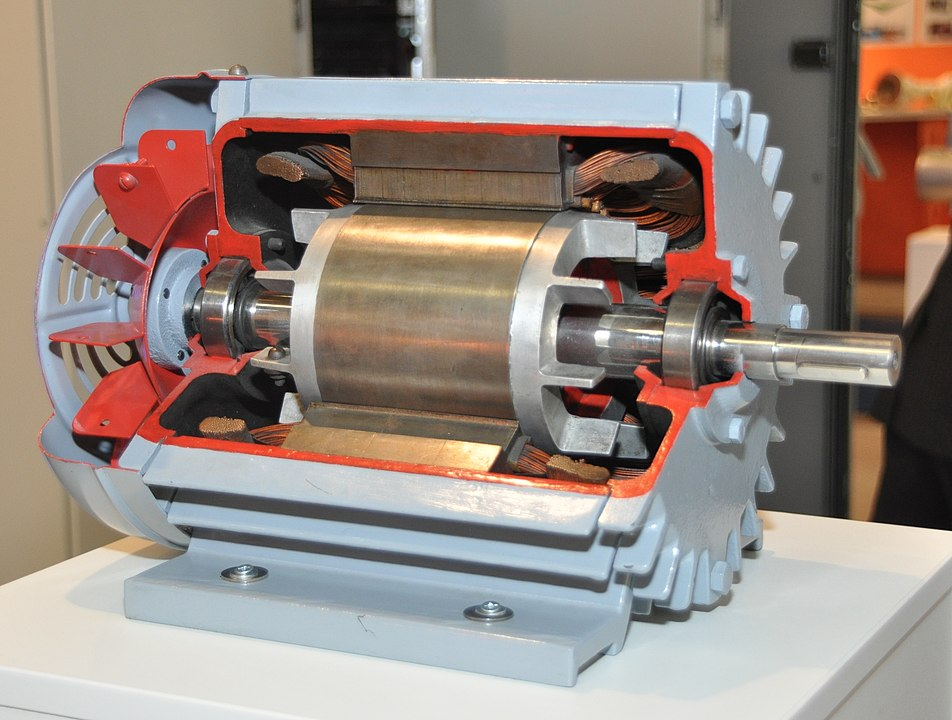
\includegraphics[width=5cm]{wikimedia-induction-motor.jpeg}\\
    {\footnotesize Source: S.J.~de~Ward, Wikimedia CC BY-SA 3.0}\\
    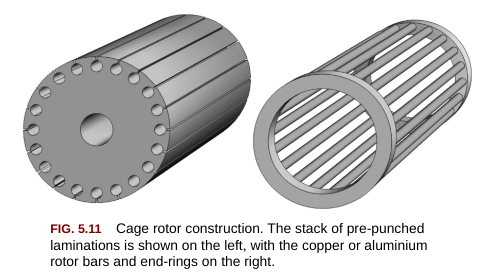
\includegraphics[width=5cm]{HD-fig5_11.png}\\
    {\footnotesize Source: Hughes and Drury}\\
  \end{center}

\end{frame}

\note{%
  - Construction of an induction motor
  - Stator and  rotor
  - Stator with slots for the stator windings
  - Stator with cooling fins
  - Rotor of cage type. Conductor rods, short-circuited at the end
  - Cooling fan, also rotor with small fins protruding to improve cooling of the rotor
}

\begin{frame}{Important concepts}

  \begin{description}
    \item[Rotating magnetic field] The 3-phase stator windings causes a magnetic flux wave to travel around the air gap at synchronous speed, $N_s$.
    \item[Slip] For torque to be produced, the rotor must rotate at speed $N < N_s$. 
    \item[Induced e.m.f and current] The flux wave cutting the rotor conductors induces an e.m.f, and hence a current.
    \item[Torque production] The rotor current interacts with the stator flux.
    \item[Rotor's effect on stator] The rotor flux opposes the stator flux.
  \end{description}

\end{frame}


\begin{frame}{The traveling flux wave of a four-pole motor}

  \begin{center}
    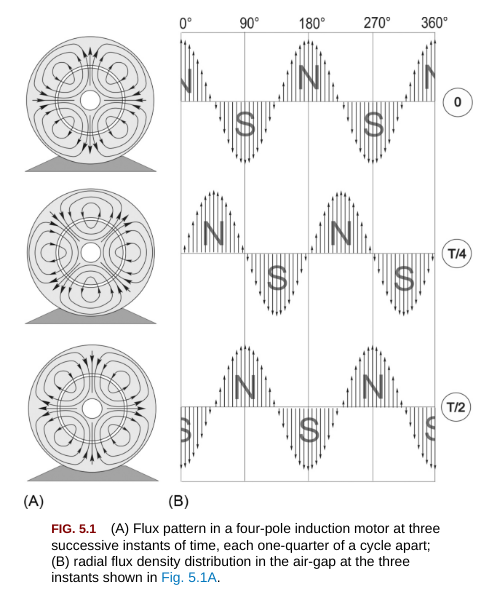
\includegraphics[width=6cm]{HD-fig5_1.png}\\
    {\footnotesize Source: Hughes and Drury}
  \end{center}

\end{frame}

\note{%
  - 
}

% ---------------------------------------------------------
%
% Stator with slots, two slots per phase.
% Pulsating current. 
%
% ---------------------------------------------------------

\begin{frame}{Magnetic field generated by the stator winding currents}

  \begin{center}

    \begin{animateinline}[controls,autoplay,loop]{20}
      \multiframe{30}{n=1+12}{
        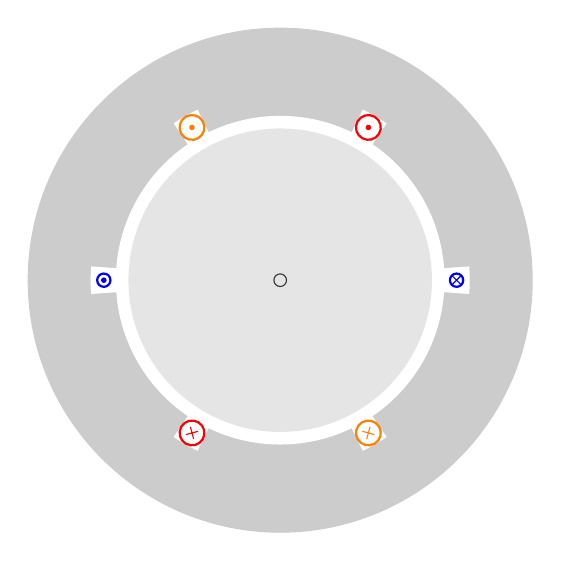
\begin{tikzpicture}[scale=0.4, transform shape]

          \stator{\statorouter}{\statorinner}{6}
          \rotor{\rotorradius}{\conductorradius}{0}
          \statorcurrent{\n}{\statorinner}{2}
      \end{tikzpicture}    
      }
    \end{animateinline}
  \end{center}
  
\end{frame}


% ---------------------------------------------------------
%
% Stator with slots, two slots per phase.
% Pulsating current. 
% Flux wave, one phase only
% ---------------------------------------------------------
\begin{frame}{Magnetic field generated by the stator winding currents}

  Flux density in the air gap shown for one phase only.
  
  \begin{center}

    \begin{animateinline}[controls,autoplay,loop]{20}
      \multiframe{30}{n=1+12}{
        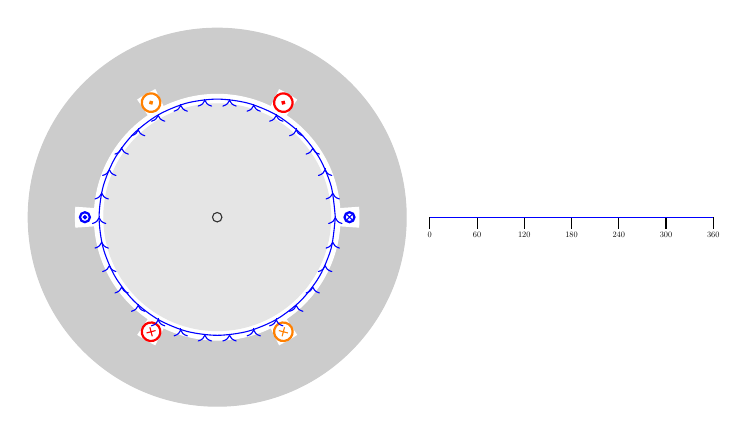
\begin{tikzpicture}[scale=0.3, transform shape]

          \begin{scope}[xshift = 8cm,]
            \pgfmathsetmacro{\axl}{12}
            \draw[] (0 cm, 0) -- (\axl cm, 0);
            \foreach \ax in {0, 60, 120, ..., 360} {
              \pgfmathsetmacro{\axx}{\ax*\axl/360.0)}
              \draw (\axx cm, 0) -- (\axx cm, -0.5) node[below] {\ax};
            }
            \foreach \rr/\ph/\clr in {0/0/blue} {
              \pgfmathsetmacro{\aa}{2*sin(\n + \ph)}
              \draw[\clr, domain=0:360, smooth, variable=\t]
              plot ( { \t*\axl/360.0 }, {-\aa*cos(\t - 90 - \rr)} );
           }

          \end{scope}

          \begin{scope}[xshift=-1cm,]

          \stator{\statorouter}{\statorinner}{6}
          \rotor{\rotorradius}{\conductorradius}{0}
          \statorcurrent{\n}{\statorinner}{2}
          \foreach \ph/\clr in {0/blue} {
            \fluxwave{\n}{\ph}{\clr}{30}
          }
        \end{scope}

          
        \end{tikzpicture}    
      }
    \end{animateinline}
  \end{center}
  What are the factors that determine the amplitude of the air gap flux density?
\end{frame}

\note{%
  - 
}

% ---------------------------------------------------------
%
% Stator with slots, two slots per phase.
% Pulsating current. 
% Flux wave. Three phases
% ---------------------------------------------------------
\begin{frame}{Magnetic field generated by the stator winding currents}

  \begin{center}

    \begin{animateinline}[controls,autoplay,loop]{20}
      \multiframe{30}{n=1+12}{
        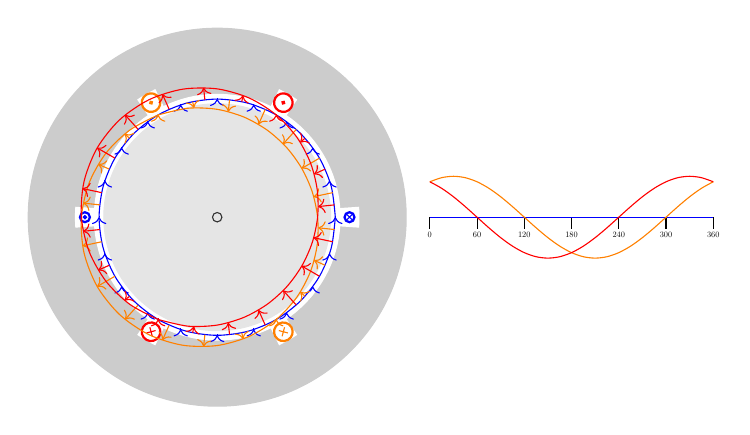
\begin{tikzpicture}[scale=0.3, transform shape]

          \begin{scope}[xshift = 8cm,]
            \pgfmathsetmacro{\axl}{12}
            \draw[] (0 cm, 0) -- (\axl cm, 0);
            \foreach \ax in {0, 60, 120, ..., 360} {
              \pgfmathsetmacro{\axx}{\ax*\axl/360.0)}
              \draw (\axx cm, 0) -- (\axx cm, -0.5) node[below] {\ax};
            }
            \foreach \rr/\ph/\clr in {0/0/blue, 120/120/orange, -120/-120/red} {
              \pgfmathsetmacro{\aa}{2*sin(\n + \ph)}
              \draw[\clr, domain=0:360, smooth, variable=\t]
              plot ( { \t*\axl/360.0 }, {-\aa*cos(\t - 90 - \rr)} );
           }

          \end{scope}

          \begin{scope}[xshift=-1cm,]

            
          \stator{\statorouter}{\statorinner}{6}
          \rotor{\rotorradius}{\conductorradius}{0}
          \statorcurrent{\n}{\statorinner}{2}
          \foreach \ph/\clr in {0/blue, 120/orange, -120/red} {
            \fluxwave{\n}{\ph}{\clr}{20}
          }
        \end{scope}

          
        \end{tikzpicture}    
      }
    \end{animateinline}
  \end{center}
  There is an apparent direction of rotation. Which is it? How can we change the direction?
\end{frame}

%\end{document}

% ---------------------------------------------------------
%
% Stator with slots, two slots per phase.
% Pulsating current. 
% Flux wave. Three phases and resulting wave
% ---------------------------------------------------------
\begin{frame}{The air gap flux wave}

  The flux wave travels at the synchronous speed
  \( N_s = \frac{120f}{p}\, \text{rpm},\) w.r.t.~the stator,
  where $f$ is the frequency of the AC power supply and $p$ is the pole number.
  
  \begin{center}

    \begin{animateinline}[controls,autoplay,loop]{20}
      \multiframe{30}{n=1+12}{
        \begin{tikzpicture}[scale=0.3, transform shape]

          \begin{scope}[xshift = 8cm,]
            \pgfmathsetmacro{\axl}{12}
            \draw[] (0 cm, 0) -- (\axl cm, 0);
            \foreach \ax in {0, 60, 120, ..., 360} {
              \pgfmathsetmacro{\axx}{\ax*\axl/360.0)}
              \draw (\axx cm, 0) -- (\axx cm, -0.5) node[below] {\ax};
            }
            \foreach \rr/\ph/\clr in {0/0/blue, 120/120/orange, -120/-120/red} {
              \pgfmathsetmacro{\aa}{2*sin(\n + \ph)}
              \draw[\clr!60, domain=0:360, smooth, variable=\t]
              plot ( { \t*\axl/360.0 }, {-\aa*cos(\t - 90 - \rr)} );
            }
            
            \draw[black!80, domain=0:360, smooth, variable=\t]
            plot ( { \t*\axl/360.0 }, {-2*(sin(\n)*cos(\t - 90 - 0) + sin(\n+120)*cos(\t - 90 - 120) + sin(\n-120)*cos(\t - 90 + 120)) } );

          \end{scope}

          \begin{scope}[xshift=-1cm,]

          \stator{\statorouter}{\statorinner}{6}
          \rotor{\rotorradius}{\conductorradius}{0}
          \statorcurrent{\n}{\statorinner}{2}
          \foreach \ph/\clr in {0/blue!50, 120/orange!50, -120/red!50} {
            \fluxwave{\n}{\ph}{\clr}{0}
          }

          % The resulting wave from adding the wave generated by the three phases
          \pgfmathsetmacro{\airgap}{\airgapradius/10}
          \draw[black!80, domain=0:360, samples=180, smooth, variable=\t]
            plot ( { (\airgap + ( sin(\n)*cos(\t - 90 - 0) + sin(\n+120)*cos(\t - 90 - 120) + sin(\n-120)*cos(\t - 90 + 120)))*cos(\t)}, {(\airgap + (sin(\n)*cos(\t - 90 - 0) + sin(\n+120)*cos(\t - 90 - 120) + sin(\n-120)*cos(\t - 90 + 120)))*sin(\t) });

        \end{scope}

          
        \end{tikzpicture}    
      }
    \end{animateinline}
  \end{center}
  What is the synchronous speed of a 8-pole motor supplied by 50Hz AC?
\end{frame}

%\end{document}

% ---------------------------------------------------------
%
% 4-pole Stator with slots, two slots per phase.
% Pulsating current. 
% Flux wave. Three phases and resulting wave
% ---------------------------------------------------------
\begin{frame}{The air gap flux wave for a 4-pole motor}

  \begin{center}

    \begin{animateinline}[controls,autoplay,loop]{20}
      \multiframe{30}{n=1+12}{
        \begin{tikzpicture}[scale=0.3, transform shape]

          \begin{scope}[xshift = 8cm,]
            \pgfmathsetmacro{\axl}{12}
            \draw[] (0 cm, 0) -- (\axl cm, 0);
            \foreach \ax in {0, 60, 120, ..., 360} {
              \pgfmathsetmacro{\axx}{\ax*\axl/360.0)}
              \draw (\axx cm, 0) -- (\axx cm, -0.5) node[below] {\ax};
            }
            \foreach \rr/\ph/\clr in {0/0/blue, 120/120/orange, -120/-120/red} {
              \pgfmathsetmacro{\aa}{2*sin(\n + \ph)}
              \draw[\clr!40, domain=0:720, smooth, variable=\t]
              plot ( { \t*\axl/360.0/2 }, {-\aa*cos(\t - 90 - \rr)} );
            }
            
            \draw[black!80, domain=0:720, smooth, variable=\t]
            plot ( { \t*\axl/360.0/2 }, {-2*(sin(\n)*cos(\t - 90 - 0) + sin(\n+120)*cos(\t - 90 - 120) + sin(\n-120)*cos(\t - 90 + 120)) } );

          \end{scope}

          \begin{scope}[xshift=-1cm,]

            \stator{\statorouter}{\statorinner}{12}
            \rotor{\rotorradius}{\conductorradius}{0}

            \statorcurrent{\n}{\statorinner}{4}

            \fourpolefluxwave{\n}{0}{black!80}
          \end{scope}

          
        \end{tikzpicture}    
      }
    \end{animateinline}
  \end{center}
\end{frame}

%\end{document}

\begin{frame}{E.m.f.~generated by a moving magnetic field}
\begin{center}
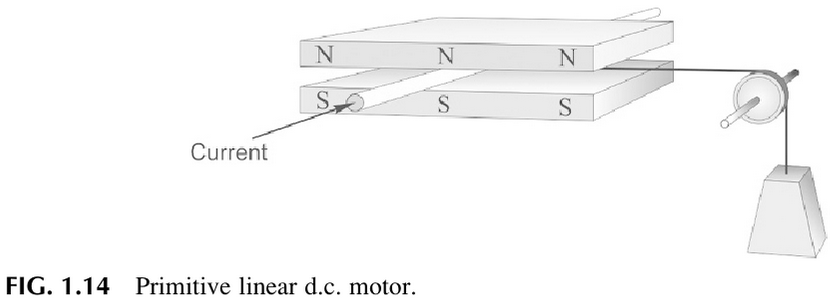
\includegraphics[width=5cm]{HD-fig1_14.png}
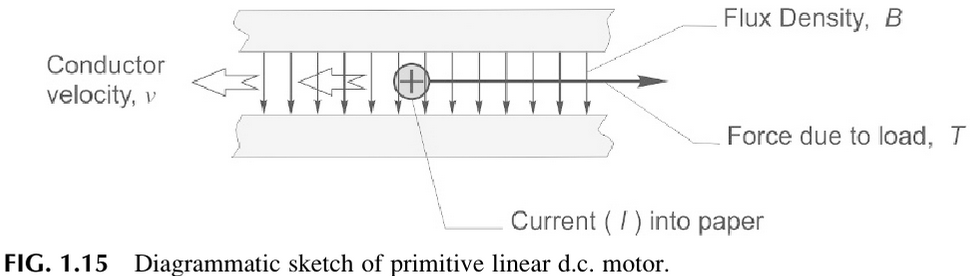
\includegraphics[width=5cm]{HD-fig1_15.png}\\
{\footnotesize Source: Hughes and Drury}
\end{center}

In the primitive linear motor with conductor moving at velocity $v$ w.r.t~ the magnetic field, the e.m.f.~is proportional to the velocity $v$ and the flux density $B$.

\end{frame}


% ---------------------------------------------------------
%
% Stator without slots, Rotor with cage.
% Traveling flux wave.
%---------------------------------------------------------
\begin{frame}{Slip}

  When motoring, the rotor rotates at speed $N =(1-s)N_s< N_s$, where the slip is defined as $s=\frac{N_s-N}{N_s}$. 
  
  \begin{center}

    \begin{animateinline}[controls,autoplay,loop]{20}
      \multiframe{60}{n=1+6}{
        \begin{tikzpicture}[scale=0.3, transform shape]

          \begin{scope}[xshift = 8cm,]
            \pgfmathsetmacro{\axl}{12}
            \draw[] (0 cm, 0) -- (\axl cm, 0);
            \foreach \ax in {0, 60, 120, ..., 360} {
              \pgfmathsetmacro{\axx}{\ax*\axl/360.0)}
              \draw (\axx cm, 0) -- (\axx cm, -0.5) node[below] {\ax};
            }
            \draw[black!80, domain=0:720, smooth, variable=\t]
            plot ( { \t*\axl/360.0/2 }, {-2*(sin(\n)*cos(\t - 90 - 0) + sin(\n+120)*cos(\t - 90 - 120) + sin(\n-120)*cos(\t - 90 + 120)) } );

          \end{scope}

          \begin{scope}[xshift=-1cm,]

            \stator{\statorouter}{\statorinner}{12}

            %\statorcurrent{\n}{\statorinner}{4}

            \pgfmathsetmacro{\rrangle}{-\n/3}
            \begin{scope}[rotate=\rrangle]
              \rotor{\rotorradius}{\conductorradius}{3}
            \end{scope}


            \fourpolefluxwave{\n}{20}{black!80}
            
        \end{scope}

          
        \end{tikzpicture}    
      }
    \end{animateinline}
  \end{center}
  The synchronus speed of a 4-pole motor supplied with 60Hz AC is $N_s = 1800$ rpm. The motor is observed to rotate at 1750 rpm. What is the slip?
  
\end{frame}

\end{document}


